%# -*- coding: utf-8-unix -*-
%%==================================================
%% thesis.tex
%%==================================================

% 双面打印
\documentclass[bachelor, openright, twoside]{sjtuthesis}
% \documentclass[bachelor, openany, oneside, submit]{sjtuthesis}
% \documentclass[master, review]{sjtuthesis}
% \documentclass[%
%   bachelor|master|doctor|coursepaper, % 必选项,分别是学士,硕士,博士学位论文以及课程论文
%   fontset=fandol|windows|mac|ubuntu|adobe|founder, % 字体选项
%   oneside|twoside,        % 单面打印,双面打印(奇偶页交换页边距,默认)
%   openany|openright,      % 可以在奇数或者偶数页开新章|只在奇数页开新章(默认)
%   english,                % 启用英文模版
%   review,     % 盲审论文,隐去作者姓名、学号、导师姓名、致谢、发表论文和参与的项目
%   submit      % 定稿提交的论文,插入签名扫描版的原创性声明、授权声明
% ]

% 逐个导入参考文献数据库
\addbibresource{bib/thesis.bib}
% \addbibresource{bib/chap2.bib}

%# -*- coding: utf-8-unix -*-
% !TEX program = xelatex
% !TEX root = ../thesis.tex
% !TEX encoding = UTF-8 Unicode
%TC:ignore
\title{面向多路口交通信号灯控制的深度强化学习算法}
\author{陈诧姹}
\advisor{张伟楠}
% \coadvisor{某某教授}
\defenddate{2019年6月10日}
\coursename{某某课程}
\school{上海交通大学}
\institute{电子信息与电气工程学院}
\studentnumber{515021910302}
\cnacademicdegree{工学学士}
\major{计算机科学与技术}
\keywords{上海交大, 饮水思源, 爱国荣校}

\englishtitle{Deep reinforcement learning for multi-intersection traffic signal control}
\englishauthor{\textsc{Chacha Chen}}
\englishadvisor{Prof. \textsc{Weinan Zhang}}
% \englishcoadvisor{Prof. \textsc{Uom Uom}}
\englishschool{Shanghai Jiao Tong University}
\englishinstitute{\textsc{Depart of Computer Sience and Engineering, School of Electronic Information and Electrical Engineering} \\
  \textsc{Shanghai Jiao Tong University} \\
  \textsc{Shanghai, P.R.China}}
\englishinstitutemaster{Depart of Computer Sience and Engineering, \\ School of Electronic Information and Electrical Engineering}
\englishmajor{A Very Important Major}
\englishdate{Dec. 17th, 2014}
\enacademicdegree{Bachelor of Engineering}
\englishstudentid{515021910302}
\englishkeywords{SJTU, bachelor thesis, XeTeX/LaTeX template}
%TC:endignore
  % NOTE: the enclosed commands must be executed in preamble

\begin{document}

% 无编号内容:中英文论文封面、授权页
\maketitle
\makeatletter

\ifsjtu@coursepaper
% 摘要 部分课程论文需要,可以自行选择添加或者去除
% %# -*- coding: utf-8-unix -*-
% !TEX program = xelatex
% !TEX root = ../thesis.tex
% !TEX encoding = UTF-8 Unicode
%%==================================================
%% abstract.tex for SJTU Master Thesis
%%==================================================

\begin{abstract}


\end{abstract}

\begin{englishabstract}


\end{englishabstract}



% 目录 部分课程论文需要,可以自行选择添加或者去除
% \tableofcontents

\else
  \ifsjtu@submit\relax
    \includepdf{pdf/original.pdf}
    \cleardoublepage
    \includepdf{pdf/authorization.pdf}
    \cleardoublepage
  \else
    \ifsjtu@review\relax
    % exclude the original claim and authorization
    \else
      \makeDeclareOriginal
      \makeDeclareAuthorization
    \fi
  \fi
  \frontmatter % 使用罗马数字对前言编号

  % 摘要
  %# -*- coding: utf-8-unix -*-
% !TEX program = xelatex
% !TEX root = ../thesis.tex
% !TEX encoding = UTF-8 Unicode
%%==================================================
%% abstract.tex for SJTU Master Thesis
%%==================================================

\begin{abstract}


\end{abstract}

\begin{englishabstract}


\end{englishabstract}



  % 目录、插图目录、表格目录
  \tableofcontents
  \listoffigures
  \addcontentsline{toc}{chapter}{\listfigurename}     % 将插图目录加入全文目录
  \listoftables
  \addcontentsline{toc}{chapter}{\listtablename}      % 将表格目录加入全文目录
  \listofalgorithms
  \addcontentsline{toc}{chapter}{\listalgorithmname}  % 将算法目录加入全文目录

  \include{tex/symbol} % 主要符号、缩略词对照表
\fi

\makeatother
\mainmatter % 使用阿拉伯数字对正文编号

% 正文内容
% introduction.tex

\section{Introduction}
\label{sec:introduction}
Traffic congestion is a growing problem that continues to plague urban areas with negative outcomes to both the traveling public and society as a whole. These negative outcomes will only grow over time as more people flock to urban areas. In 2014, traffic congestion costs Americans over \$160 billion in lost productivity and wasted over 3.1 billion gallons of fuel~\cite{Econ14}. Traffic congestion was also attributed to over 56 billion pounds of harmful CO2 emissions in 2011~\cite{schrank20152015}. 
In the European Union, the cost of traffic congestion was equivalent to 1\% of the entire GDP~\cite{schrank2012tti}.
Mitigating congestion would have significant economic, environmental and societal benefits.
Signalized intersections are one of the most prevalent bottleneck types in urban environments, and thus traffic signal control plays a vital role in urban traffic management.

\begin{figure}[t]
\centering
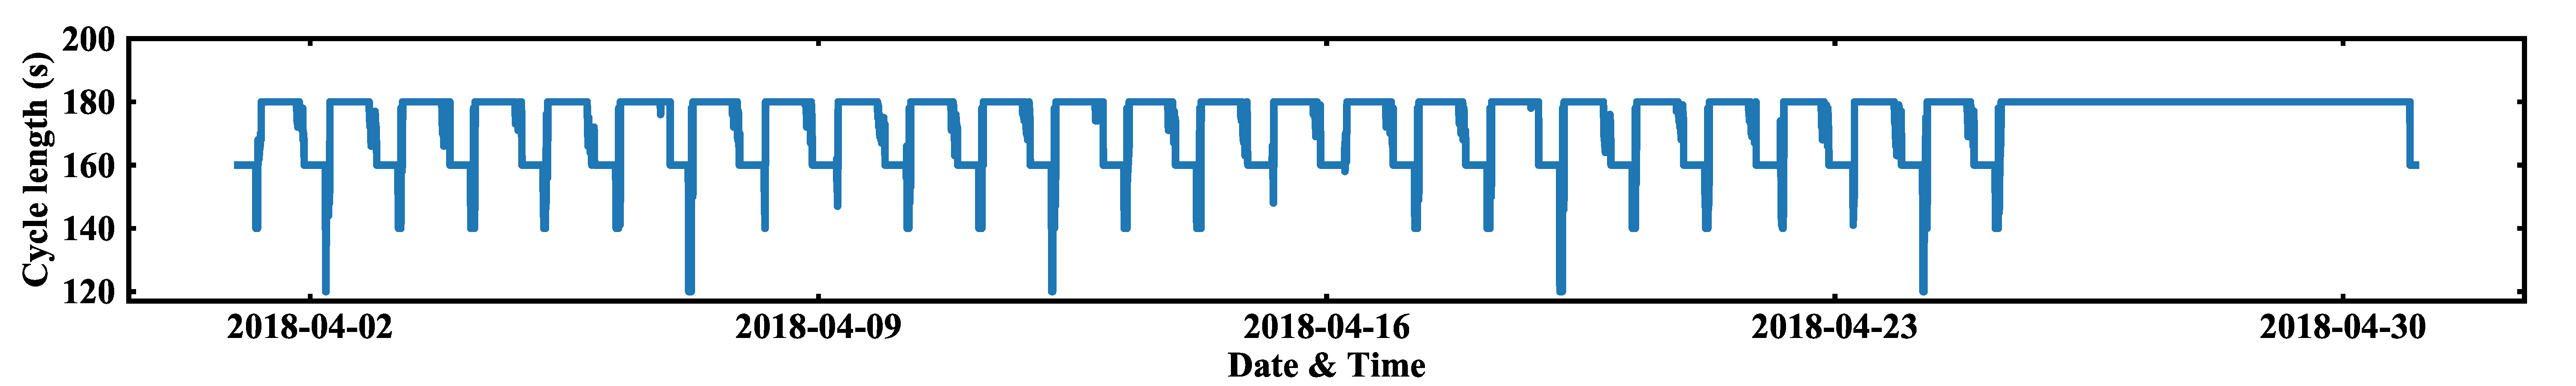
\includegraphics[width=0.99\textwidth]{figures/timing.pdf} 
\caption{Traffic signal timing in a city. The cycle length rarely changes.}
\label{fig:timing}
\end{figure}


\subsection{Current Situation}
In many modern cities today, the widely-used adaptive traffic signal control systems such as SCATS~\cite{SCATS} and SCOOT~\cite{hunt1981scoot,hunt1982scoot} heavily rely on manually designed traffic signal plans. Such manually set traffic signal plans are designed to be dynamically selected according to the traffic volume detected by loop sensors. However, many intersections do not have loop sensors installed or the loop sensors are poorly maintained. Moreover, the loop sensors are activated only when vehicles pass through them, thus they can only provide partial information about the vehicle through them. As a result, the signal cannot perceive and react to the real-time traffic patterns, and engineers need to manually change the traffic signal timings in the signal control system under certain traffic condition scenarios. Figure~\ref{fig:timing} shows the traffic signal timing at an intersection in a city of China and the traffic signal timing rarely changes regardless of the real traffic changes throughout the day.


\subsection{Opportunities}
\emph{First, today we have much richer information that can be collected from various sources.} Traditional traffic signal control relies on data from loop sensors, which can only sense the vehicle passing. However, new data sources are quickly becoming available that can serve as input for traffic signal control purposes. For instance, street-facing surveillance cameras used for security purposes can also provide a more detailed depiction of  the traffic situation on nearby roads -- specifically, how many cars are waiting in the lane, how many cars are taking turns, where they are located, and how fast they are traveling. In addition, large-scale trajectory data can be collected from various sources such as navigation applications (e.g., Google Maps),  ride-sharing platforms (e.g., Uber) and GPS-equipped vehicles that share information with the nearby infrastructure (e.g., connected vehicles). Such data provide us with more insight about how vehicles arrive to intersections. We have reached a stage of abundant mobility information that can describe the traffic dynamics in the city more clearly, which is an essential resource for us to improve the traffic control system.


 
\begin{figure}[htbp]
\centering
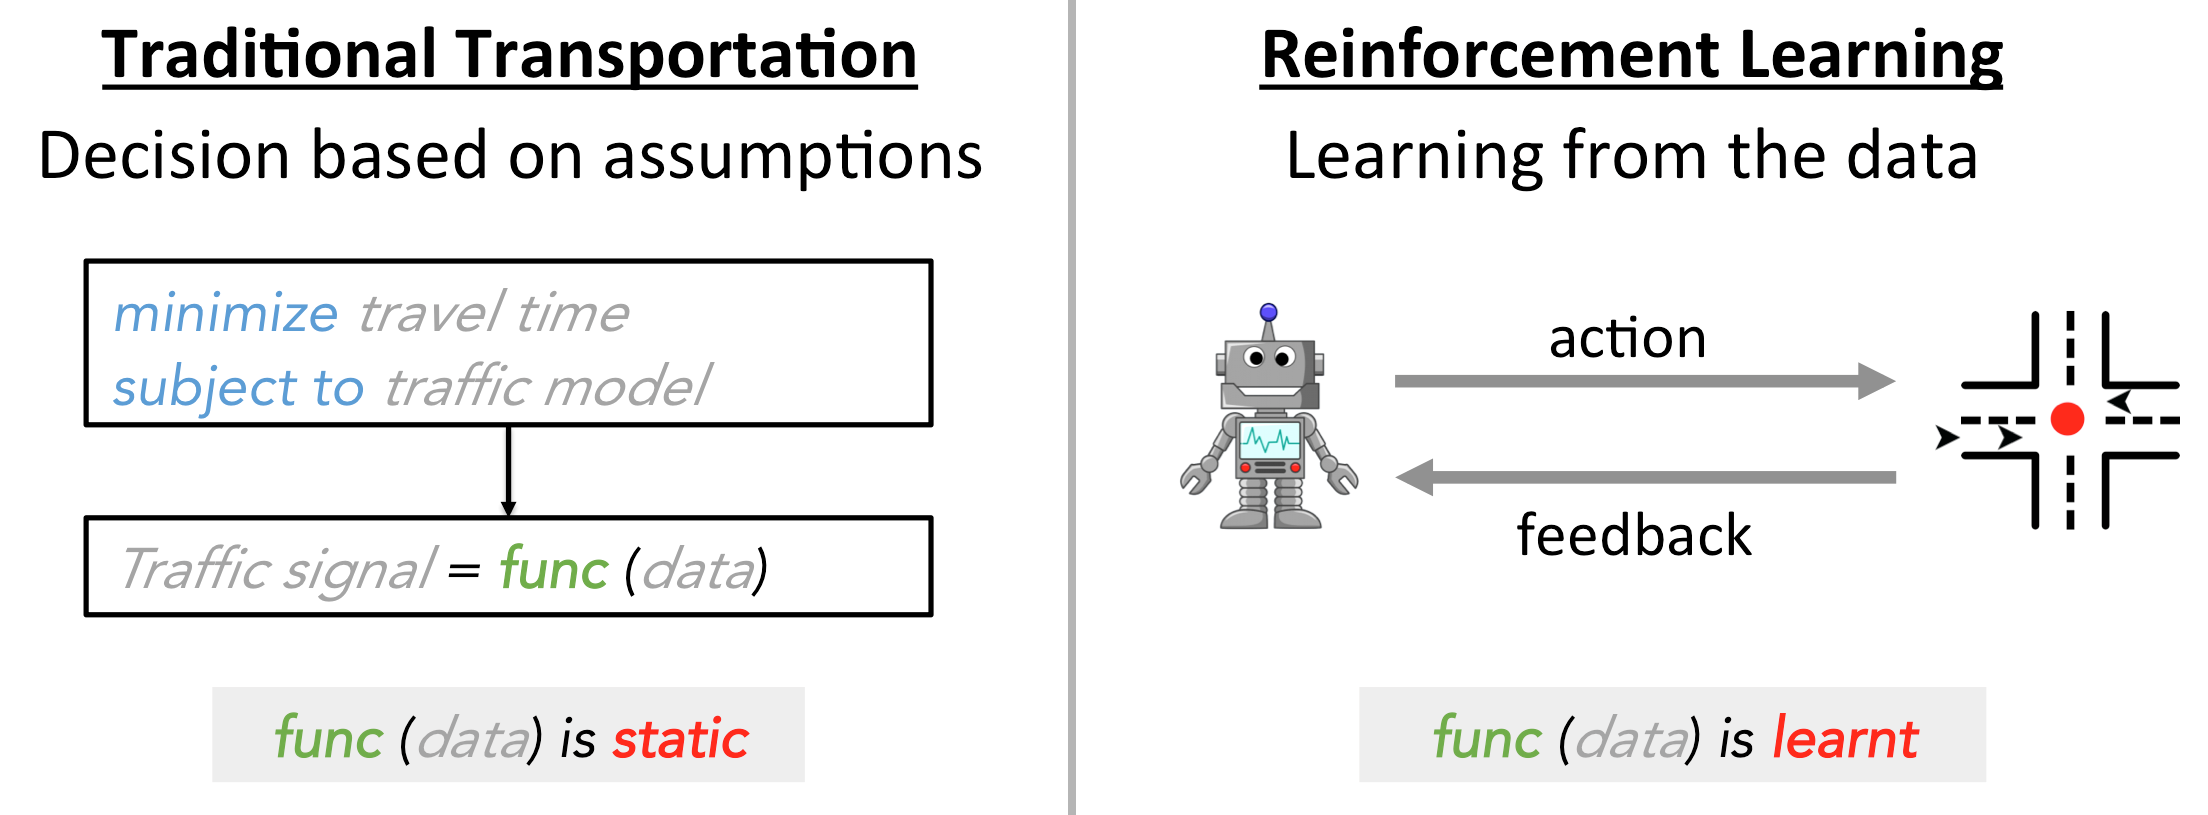
\includegraphics[width=0.7\columnwidth]{fig/optimizationvsRL.png}
\caption{Difference between traditional transportation approach and machine learning approach.}
\label{fig:optvsrl}
\end{figure}

\emph{Second, today we have much stronger computing power and advanced computational models.} The typical approach that transportation researchers take is to cast traffic signal control as an optimization problem under certain assumptions about the traffic model, e.g., vehicles come in a uniform and constant rate~\cite{RPM04}.  Various (and sometimes strong) assumptions have to be made in order to make the optimization problem tractable. The key issue here is that these assumptions deviate from the real world and often do so significantly. As we know, real-world traffic condition evolves in a complicated way, affected by many factors such as driver's preference, interactions with vulnerable road users (e.g. pedestrians, cyclists, etc.), weather and road conditions, just to name a few. These factors can hardly be fully described in a traffic model.


On the other hand, machine learning techniques can directly learn from the observed data without making unrealistic assumptions about the model. However, typical supervised learning does not apply here because existing traffic signal control systems follow pre-defined signal plans so we do not have enough training data to differentiate good and bad traffic signal plan strategies. Instead, we have to first take actions to change the signal plans and then learn from the outcomes. This trial-and-error approach is also the core idea of reinforcement learning (RL). In essence, an RL system generates and executes different strategies (e.g., for traffic signal control) based on the current environment. It will then learn and adjust the strategies based on the feedback from the environment. This reveals the biggest difference between transportation approaches and our RL approaches, which is illustrated in Figure~\ref{fig:optvsrl}: in traditional transportation research, the model $func(data)$ is static; in reinforcement learning, the model is dynamically learned through trial-and-error in the real environment.





\include{tex/example}
\include{tex/faq}
\include{tex/summary}

\appendix % 使用英文字母对附录编号

% 附录内容,本科学位论文可以用翻译的文献替代。
\include{tex/app_setup}
\include{tex/app_eq}
\include{tex/app_cjk}
\include{tex/app_log}

\backmatter % 文后无编号部分

% 参考资料
\printbibliography[heading=bibintoc]

% 致谢、发表论文、申请专利、参与项目、简历
% 用于盲审的论文需隐去致谢、发表论文、申请专利、参与的项目
\makeatletter

\ifsjtu@coursepaper
\else

  % "研究生学位论文送盲审印刷格式的统一要求"
  % http://www.gs.sjtu.edu.cn/inform/3/2015/20151120_123928_738.htm

  % 盲审删去删去致谢页
  \ifsjtu@review\relax\else
    %# -*- coding: utf-8-unix -*-
% !TEX program = xelatex
% !TEX root = ../thesis.tex
% !TEX encoding = UTF-8 Unicode
%TC:ignore
\begin{thanks}
I must express my very profound gratitude to my co-workers and advisors for providing me with unfailing support and continuous encouragement throughout my years of study and through the process of researching and writing this thesis.

\end{thanks}
%TC:endignore
         % 致谢
  \fi

  \ifsjtu@bachelor
    % 学士学位论文要求在最后有一个英文大摘要,单独编页码
    %# -*- coding: utf-8-unix -*-
% !TEX program = xelatex
% !TEX root = ../thesis.tex
% !TEX encoding = UTF-8 Unicode
\begin{bigabstract}


\end{bigabstract}
  \else
    % 盲审论文中,发表学术论文及参与科研情况等仅以第几作者注明即可,不要出现作者或他人姓名
    \ifsjtu@review\relax
      \include{tex/pubreview}
      \include{tex/projectsreview}
    \else
      \include{tex/pub}       % 发表论文
      \include{tex/projects}  % 参与的项目
      % \include{tex/patents}   % 申请专利
      \include{tex/resume}    % 个人简历
    \fi
  \fi
\fi

\makeatother

\end{document}
